%%%%%%%%%%%%%%%%%%%%%%%%%%%%%%%%%%%%%%%%%
% Beamer Presentation
% LaTeX Template
% Version 1.0 (10/11/12)
%
% This template has been downloaded from:
% http://www.LaTeXTemplates.com
%
% License:
% CC BY-NC-SA 3.0 (http://creativecommons.org/licenses/by-nc-sa/3.0/)
%
%%%%%%%%%%%%%%%%%%%%%%%%%%%%%%%%%%%%%%%%%

%----------------------------------------------------------------------------------------
%	PACKAGES AND THEMES
%----------------------------------------------------------------------------------------

\documentclass{beamer}

\mode<presentation> {

%\usetheme{default}
%\usetheme{Antibes}
%\usetheme{Boadilla}
\usetheme{JuanLesPins}
%\usetheme{Madrid}
%\usetheme{Rochester}



% As well as themes, the Beamer class has a number of color themes
% for any slide theme. Uncomment each of these in turn to see how it
% changes the colors of your current slide theme.

%\usecolortheme{beaver}
%\usecolortheme{dolphin}
%\usecolortheme{orchid}
%\usecolortheme{rose}
%\usecolortheme{seagull}
%\usecolortheme{seahorse}
%\usecolortheme{whale}
%\usecolortheme{wolverine}

%\setbeamertemplate{footline} % To remove the footer line in all slides uncomment this line
\setbeamertemplate{footline}[frame number] % To replace the footer line in all slides with a simple slide count uncomment this line

\setbeamertemplate{navigation symbols}{} % To remove the navigation symbols from the bottom of all slides uncomment this line

\setbeamertemplate{caption}[numbered]
}

\usepackage{graphicx}
\usepackage{booktabs}
\usepackage{subfig}
\usepackage{amssymb}
\usepackage{amsmath}
\usepackage[%
	autocite    = superscript,
	backend     = bibtex,
	sortcites   = true,
	style       = numeric,
	sorting     = none,
]{biblatex}
\addbibresource{reference.bib}
\graphicspath{{./Images/}}

%----------------------------------------------------------------------------------------
%	TITLE PAGE
%----------------------------------------------------------------------------------------

\title[High speed Flight]{Learning High-Speed Flight in the Wild \autocite{high-speed-flight}}
\author{Edwin Jose George}
\institute[GCEK]{
	Guided by Dr. Rafeeque P C \\
	\medskip
	Department of Computer Science and Engineering \\
	Government College of Engineering Kannur
}
\date{\today}

\begin{document}

\begin{frame}
	\titlepage
\end{frame}

\begin{frame}{Overview}
	\tableofcontents
\end{frame}

%----------------------------------------------------------------------------------------
%	PRESENTATION SLIDES
%----------------------------------------------------------------------------------------
\section{Introduction}
\begin{frame}{Introduction}
	\begin{itemize}
		\item Quadrotors (drones) are the most agile and dynamic machines, traversing extremely complex environments at high speeds. 
		\item State of the art autonomous operation with onboard sensing and computation has been limited to low speeds.
		\item This limiting factor for autonomous agile flight in arbitrary unknown environments is the coupling of fast and robust perception with effective planning. 
	\end{itemize}
\end{frame}

\section{Problem Statement}
\begin{frame}{Problem Statement}
	To construct an end-to-end approach that directly map noisy sensory observations to collision-free trajectories in a receding-horizon \autocite{receding_horizon} fashion, with purely onboard sensing and computation. \\~\\
	
	\begin{itemize}			
		\item This direct mapping drastically reduces processing latency and increases robustness to noisy and incomplete perception. 
		
		\item The sensorimotor mapping is performed by a convolutional network.
	\end{itemize}
\end{frame}

\section{Constraints}
\begin{frame}{Constraints to meet}
	\begin{itemize}
		\item Must be robust to disturbances such as sensor noise, motion blur, and changing illumination conditions.
		\item An effective planner to find a path that is both dynamically feasible and collision-free while relying only on noisy and partial observations of the environment.
		\item The limited computational resources that are available on board, 
		\item Other factors such as aerodynamics, torque, power, reaction delays etc.
	\end{itemize}
\end{frame}


\section{Literature Review}

\begin{frame}{Traditional Methodology}
	\begin{itemize}
		\item The division of the navigation task into sub task
		\begin{itemize}
			\item Sensing
			\item Mapping
			\item Planning	
		\end{itemize} 
	
		\item Attractive from an engineering perspective because it enables parallel progress on each component and makes the overall system interpretable. 
		\item It leads to pipelines that largely neglect interactions between the different stages and thus compound errors. 
		\item Their sequential nature also introduces additional latency.
	\end{itemize}
\end{frame}

\begin{frame}{State of the art Model}
	\begin{itemize}
		\item Some works tackle only perception and build high-quality maps from imperfect measurements \autocite{fastPlanner}. 
		\item Other works focus on planning without considering perception errors. \autocite{reactive_method}
		\item Numerous systems that combine online mapping with traditional planning algorithms have been proposed to achieve autonomous flight in unknown environments.
		\begin{itemize}
			\item 3D euclidean signed distance fields
			\item Pushbroom stereo
			\item Rapid exploration with multi-rotors
		\end{itemize} 
	\end{itemize}
\end{frame}

\begin{frame}{Recent Models}
	\begin{itemize}
		\item Proposal to learn end-to-end policies directly from data without explicit mapping and planning stages. 
		\item These policies are trained by imitating a human, from experience (or stimulation). 
		\item More recent work has demonstrated that very agile control policies can be trained in simulation. 
		\item Policies produced by the last approach can successfully perform acrobatic maneuvers, but can only operate in unobstructed free space.
	\end{itemize}
\end{frame}

\begin{frame}{Taxonomy of existing approaches for drone navigation}
	\centering
	\begin{figure}
		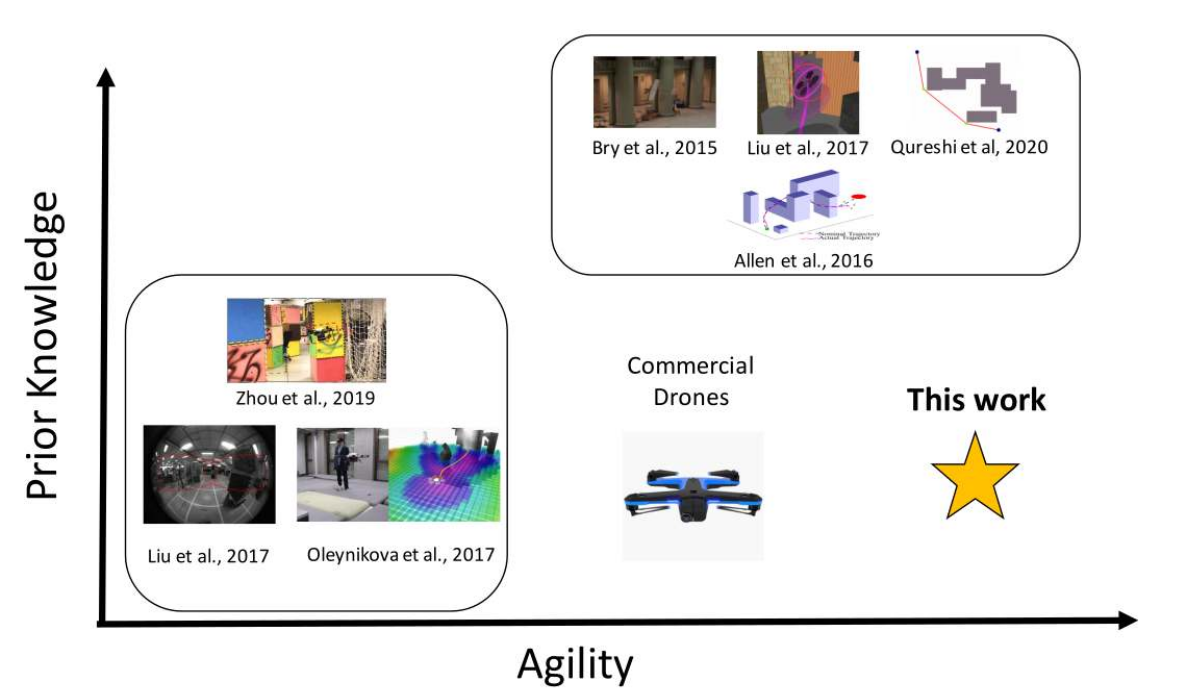
\includegraphics[height=2in]{taxonomy_navigation.png}
		\caption{Taxonomy of existing approaches for drone navigation in challenging and cluttered environments.}
	\end{figure}
\end{frame}

\section{Methodology}
\begin{frame}{Sensorimotor Policy}
	\begin{itemize}
		\item It predicts receding-horizon \autocite{receding_horizon} trajectories from on-board sensor measurements and a reference trajectory.
		
		\item Inputs
		\begin{itemize}
			\item Depth Image $d \in \mathbb{R}^{640*480}$ from Semi-Global Matching algorithm \autocite{stereoMatching}
			\item Estimate of the platform velocity $v \in \mathbb{R}^3$
			\item Attitude (rotation matrix) $q \in \mathbb{R}^9$
			\item Desired flight direction $\omega \in \mathbb{R}^3$
		\end{itemize}
	
		\item Outputs : A set of motion hypotheses with the corresponding estimated risk of collision. 
		
	\end{itemize}
\end{frame}

\begin{frame}[allowframebreaks]{The Privileged expert}
	It is a sampling-based motion planning algorithm with global planning \autocite{global_planning}.
	
	\begin{block}{Probability of trajectory}
	
	\begin{flalign}
		P(\tau | \tau_{ref},C) = & \frac{1}{Z} exp(-c(\tau, \tau_{ref},C)) \\
		Z = & \int_{\tau} P(\tau | \tau_{ref},C) 
	\end{flalign}

	\end{block}

	\newpage

	Way too complex! To approximate the density P, we use random sampling using M-H algorithm \autocite{MH_hasting}. \\~\\
	
	To decrease the dimension of the sampling space, We represent trajectory as a
	\textbf{cubic B-spline} $\tau_{bspline} \in \mathbb{R}^{3*3} $ curve with three control points and a
uniform knot vector.

\end{frame}

\begin{frame}{The Student Policy}
	\begin{itemize}
		\item It produces collision-free trajectories in real time with access only to on-board sensor measurements.
		\item Make use of pre-trained MobileNetV3 architecture \autocite{MobileNet}
		\item Perceptron network engage in combining features.
		\begin{block}{Trajectory}
			\begin{flalign}
				\mathbb{T}_n & = \{ (\tau_n^k, c_k) | \in [0, 1, ..., M-1 ]\} \\
				\tau_n^k & = [p(t_i)]_{i=1}^{10}, t_i = \frac{i}{10}
			\end{flalign}
		\end{block}
		
	\end{itemize}
	
\end{frame}

\begin{frame}{Method overview}
	\begin{figure}
		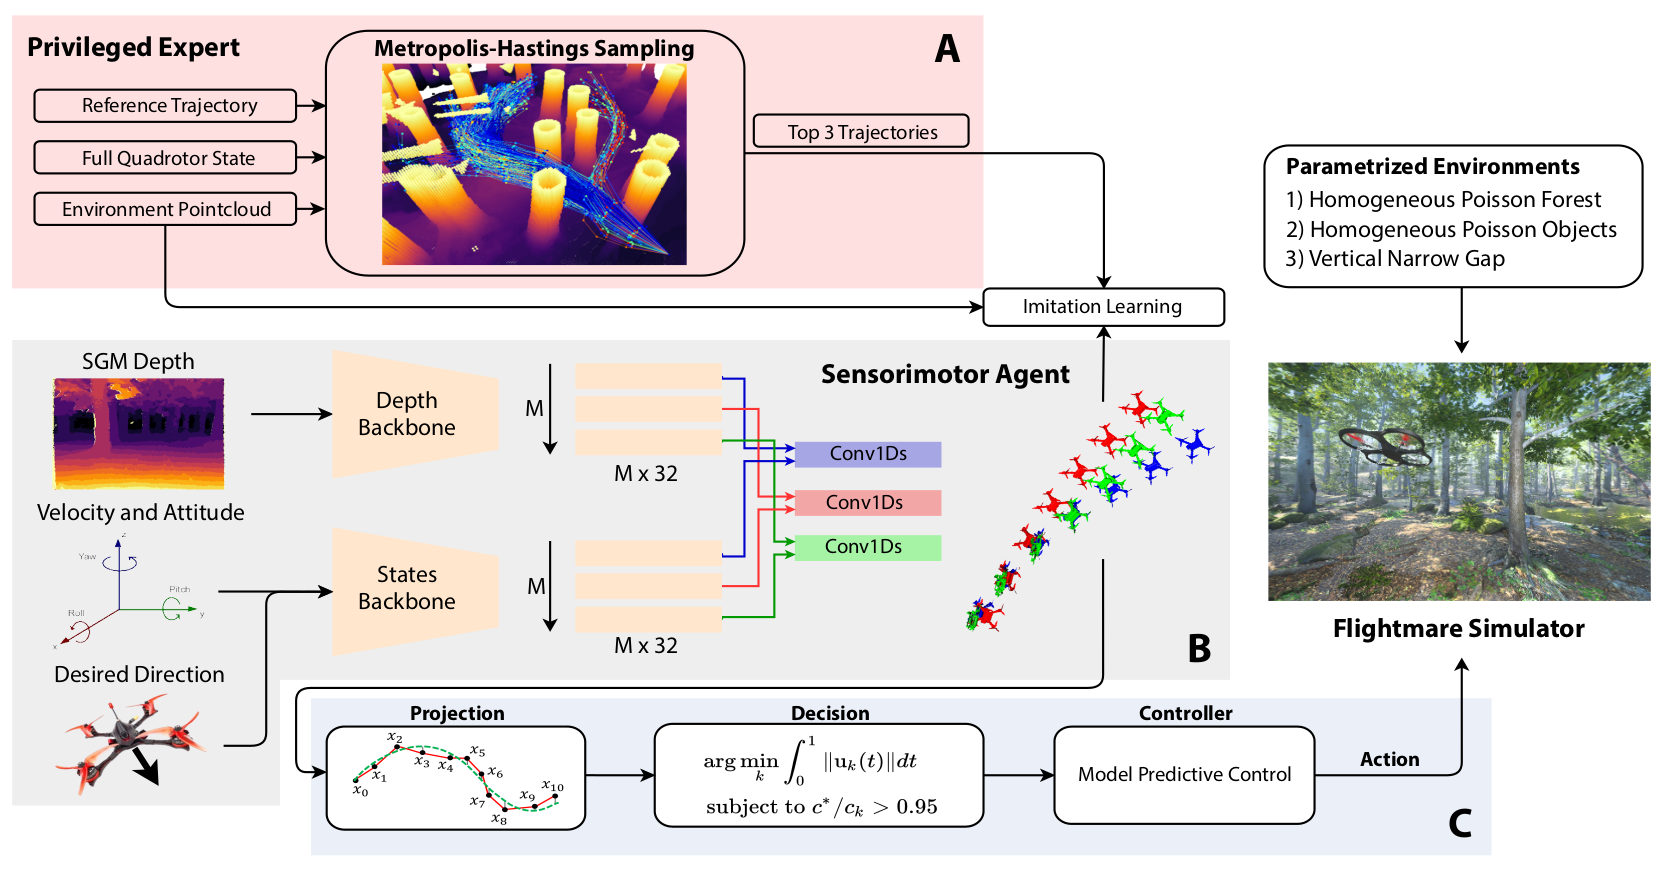
\includegraphics[width=4in]{method-overview.png}
		\caption{Overview of method}
	\end{figure}
\end{frame}

\section{Result}

\subsection{Real-world Environment}
\begin{frame}{Method of evaluation}
	'\begin{itemize}
		\item Results are confirmed in a variety of real-world environments using a \textit{custom-built physical quadrotor}
		\item Policy trained in simulation was deployed without any further adaptations.
		\item In all experiments, the drone was provided with a reference trajectory, which is not collision-free.
		\item The drone is tasked to follow that flight path and make adjustments as necessary to avoid obstacles.
		\item The performance is measured according to success rate
		\begin{itemize}
			\item The percentage of successful runs over the total number of runs
			\item A run successful if the drone reaches the goal location within a radius of 5 m without crashing.
		\end{itemize} 
	\end{itemize}
\end{frame}

\begin{frame}{Natural and Human-made environment}
	\begin{itemize}
		\item Natural Environment
		\begin{itemize}
			\item complex structure
			\item multiple options available to avoid obstacles. 
			\item A high-level understanding of the environment is necessary.
			\item Challenging illumination conditions
			\item Low texture surfaces (e.g. because of snow)
		\end{itemize}
	
		\item Human-made Environment
		\begin{itemize}
			\item Obstacles with a variety of sizes and shapes \\
			(e.g. a train, a crane, building and ruins)
			\item Limited number of flyable openings (eg. Narrow openings)
			\item Requires to initiate the avoidance maneuver well in advance.
		\end{itemize}
	\end{itemize}	
\end{frame}

\begin{frame}{Natural and Human-made environment - Graph }
	\begin{figure}
		\subfloat[Aggregate result]{
			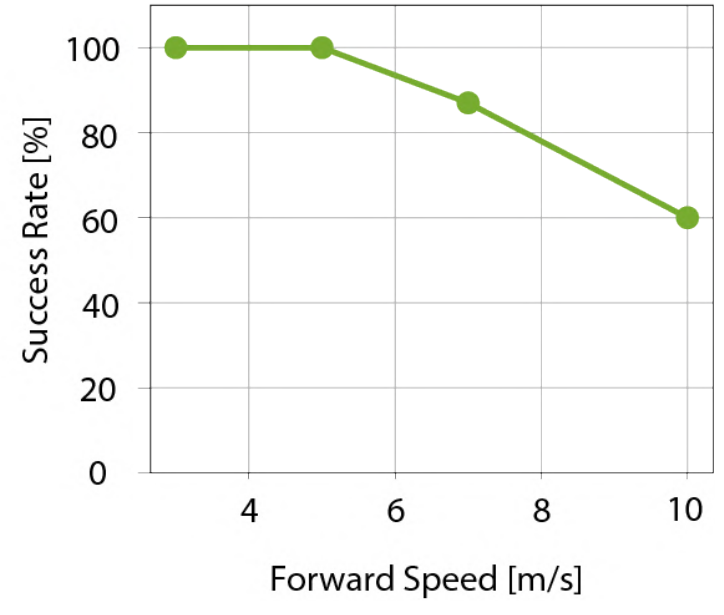
\includegraphics[width=1.5in]{natural-human-linegraph.png}
		}
		\subfloat[Individual result]{
			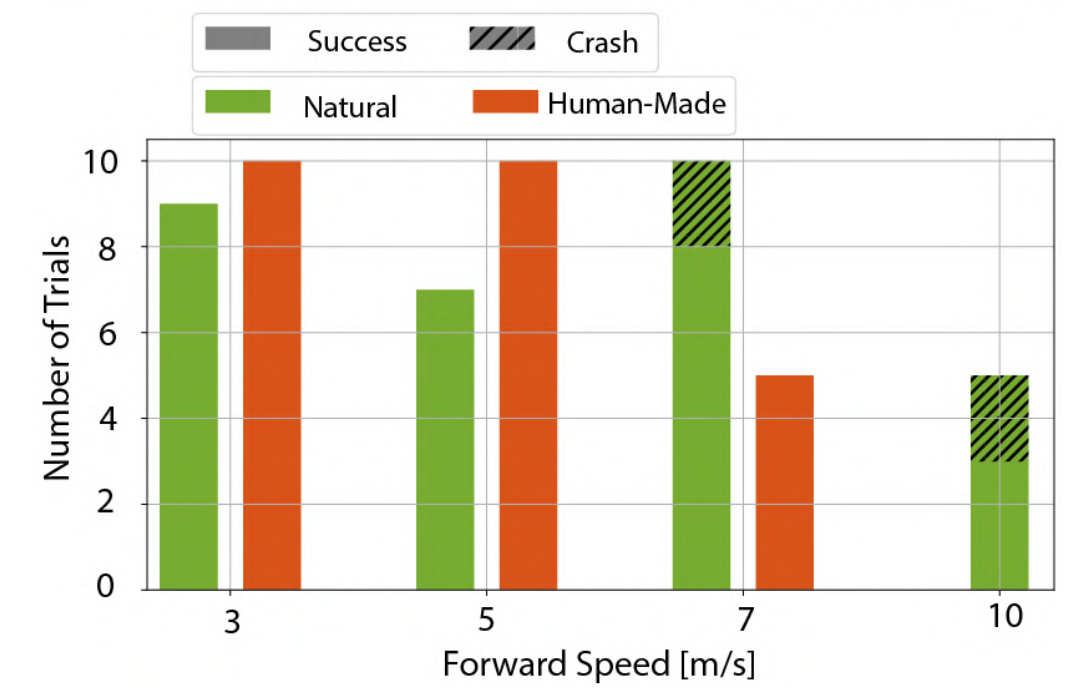
\includegraphics[width=2.5in]{natural-human-bargraph.png}
		}
		\caption{Trails on natural and human-made environment on physical drone}
	\end{figure}
\end{frame}

\subsection{Stimulated Environment}
\begin{frame}{Controlled Experiments - Comparative results}
	\begin{itemize}
		\item Two representative state-of-the-art approaches as selected as baselines for navigation in unknown environments: 
		\begin{itemize}
			\item Mapping and planning method - FastPlanner \autocite{fastPlanner}
			\item Reactive planner \autocite{reactive_method}
		\end{itemize}
	
		\item Experiments are stimulated in the \textit{Flightmare simulator} using the RotorS Gazebo plugin for physics modeling and Unity as a rendering engine.
		
	\end{itemize}
\end{frame}

\begin{frame}{Controlled Experiments - Graphs}
	\begin{figure}
		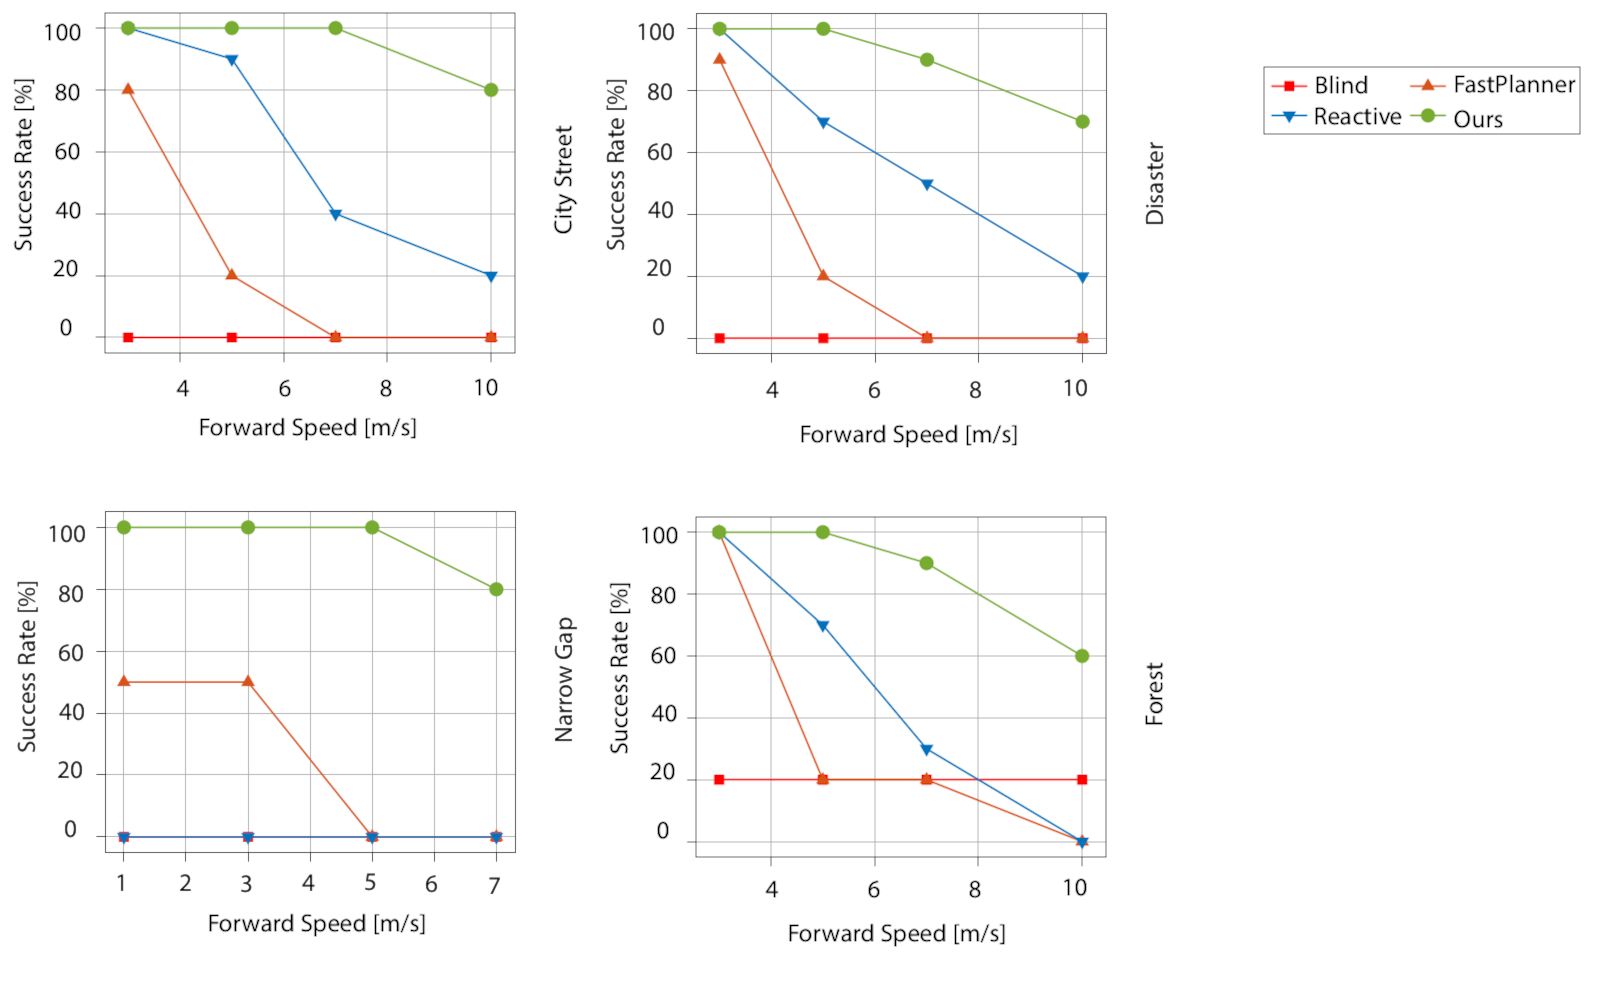
\includegraphics[width=4in]{controlled-experiments.png}
		\caption{Stimulated results}
	\end{figure}
	
\end{frame}

\begin{frame}[allowframebreaks]{The effect of latency and sensor noise}
	\begin{itemize}
		\item In this experiment, the quadrotor travels along a straight line at a constant forward speed and is required to laterally evade a single obstacle (a pole) while having only limited sensing range.
		\item The theoretical maximum speed is the speed at which the task is no longer feasible for each method. 
		\item The maximum speed depends on 
		\begin{itemize}
			\item sensing range - how far can an obstacle be accurately perceived
			\item latency of the visual sensor - the inverse of the frame rate
			\item processing latency - the time to convert an observation into motor commands.
		\end{itemize} 
	
		\pagebreak
		
		\begin{block}{Formula}
			theoretical maximum speed
			\begin{equation}
				v_{max} = \frac{s}{t_s + t_p + t_{rot} + \sqrt{\frac{2*r_{obs}}{sin(\theta)*c_{max}}}}
			\end{equation}
		\end{block}
		\item The experiment is run in two settings:
		\begin{itemize}
			\item with \textbf{ground-truth depth} information - to isolate the effect of latency on performance
			\item with \textbf{depth estimated by stereo matching}\autocite{stereoMatching} - to analyze the effect of sensing errors on performance.
		\end{itemize}
	\end{itemize}
\end{frame}

\begin{frame}{Effect of latency and noise - graphs}
	\begin{figure}
		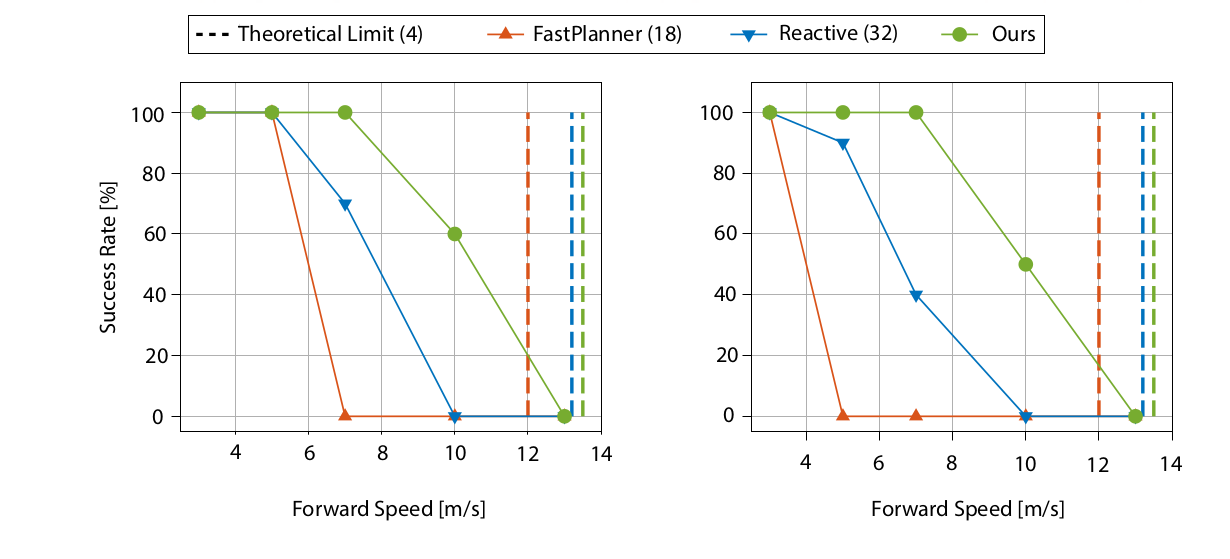
\includegraphics[width=4in]{noise-graph.png}
		\caption{The effect of sensor noise on performance. The experiment is performed on ground-truth-depth (1) and stereo-depth (2)}
	\end{figure}
\end{frame}

\begin{frame}{Effect of latency and noise - images}
	\begin{figure}
		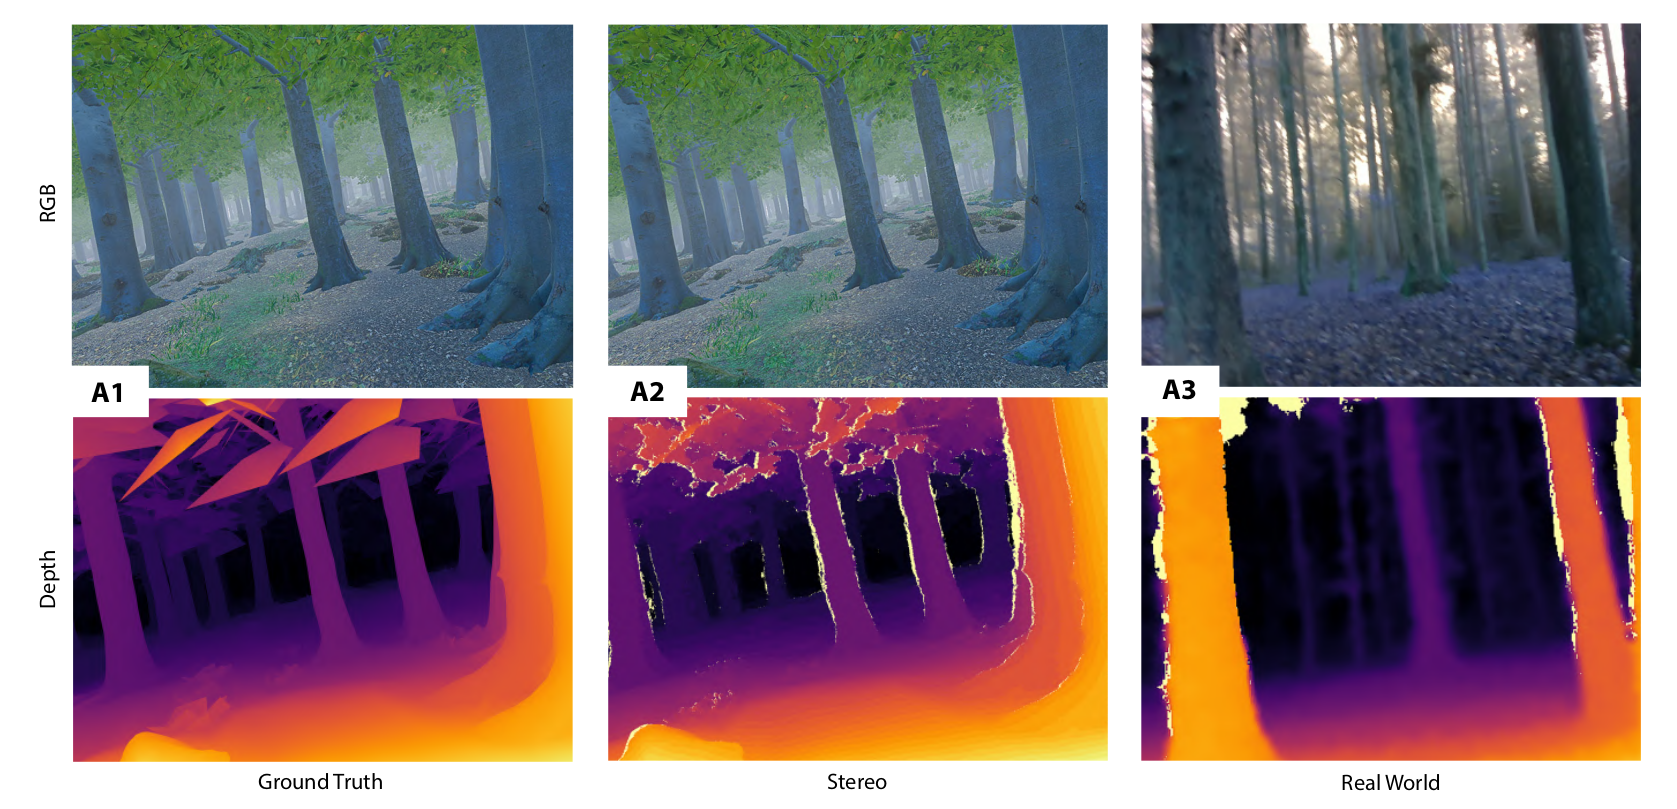
\includegraphics[width=4in]{stimulation and stereo.png}
		\caption{The image perceived by the system}
	\end{figure}
\end{frame}

\section{Conclusions}
\begin{frame}{Conclusion}
	\begin{itemize}
		\item We achieve high speed flight by training a neural network to imitate an expert with privileged information in simulation.
		
		\item Coping with the complexity of the task and to enable seamless transfer from simulation to reality, several technical contributions accounting multi-modality are proposed.
		
		\item The combination of these innovations enables the training of robust navigation policies in simulation that can be directly transferred to diverse real-world environments without any fine-tuning on real data.
	\end{itemize}
	
	
\end{frame}

\section{Future Scope}
\begin{frame}[allowframebreaks]{Opportunities for future works}
	\begin{itemize}
		\item Low success rates at average speeds of $10 ms^{-1}$ or higher in the real world. \\
		\textbf{Reason}: At higher speeds, feasible solutions require temporal consistency over a long time horizon and strong variations of the instantaneous flying speed.\\
		\textbf{Solution} : Engineering a more complex expert by specifically tailored heuristics to find approximate solutions. 
		
		\item Perception latency: Faster sensors can provide more information in smaller amount of time. This could enable further reducing sensitivity-to-noise and promote a quicker understanding of the environment. \\
		\textbf{Solution} : Use of event cameras, especially in the presence of dynamic obstacles.
		
		\item Mismatch between the simulated and physical drone in terms of dynamics and perception. \\
		\textbf{Reason} : Aerodynamics effects, motor delays, and dropping battery voltage. \\
		\textbf{Solution} : Increasing the fidelity of the simulated drone and making the policy robust to the unavoidable model mismatches.		
	\end{itemize}
	
\end{frame}

\section{References}
\begin{frame}[allowframebreaks]{References}
	\printbibliography
\end{frame}

\end{document}